% Copyright (c) 2015 Benito Palacios Sánchez - All Rights Reserved.
% Esta obra está licenciada bajo la Licencia Creative Commons Atribución 4.0
% Internacional. Para ver una copia de esta licencia, visita
% http://creativecommons.org/licenses/by/4.0/.

\section[Fan-traducciones]{Traducciones no oficiales}
\subsection{Saga Pokémon}

\begin{frame}{Traducciones no oficiales y Pokémon}
\pause
\note<1>[item]{Puesto el contexto sobre las ediciones de videojuegos, se va a pasar a explicar los resultados del estudio de la problemática identificada: las traducciones no oficiales, donde el caso más claro se da con la Saga Pokémon.}

\begin{columns}
  \begin{column}{0.6\textwidth}
    \begin{wideitemize}
        \item<+-> Franquicia de \textit{The Pokémon Company} fundada en 1995.
        Juegos desarrollados por \textit{Game Freak}.
        \note<1>[item]{Se fundó en 1995 por Satoshi Tajiri cuando diseñaba muñecos para la empresa Creatures Inc.}
        \note<1>[item]{El primer juego en 1996 rojo y verde, al año un millón de copias.}
        \note<1>[item]{Exclusivos de Nintendo. A día de hoy cuenta con merchandaising, ropa, cartas, películas, anime, manga, etc.}

        \item<+-> Segunda franquicia más exitosa a nivel mundial.
        \note<1>[item]{Solo está detras de Mario de Nintendo.}
        \note<1>[item]{En 2010 se llegaron a los 200 millones de copias vendidas. Solo la marca ganó en 2014 \$2.000 millones}

        \item<+-> Nº seguidores + retrasos en lanzamientos $\Rightarrow$ traducción no oficial.
        \note<1>[item]{Desde la salida de japón a América son 6 meses y a Europa otros 4.}
        \note<1>[item]{Traducciones dinámicas, parches cada semana, que quitan mercado.}
    \end{wideitemize}

    \note<1>{Se analizará la seguridad de 4 de los 6 videojuegos de esta saga. Se verá la evolución de la seguridad.}
  \end{column}

  \begin{column}{0.4\textwidth}
    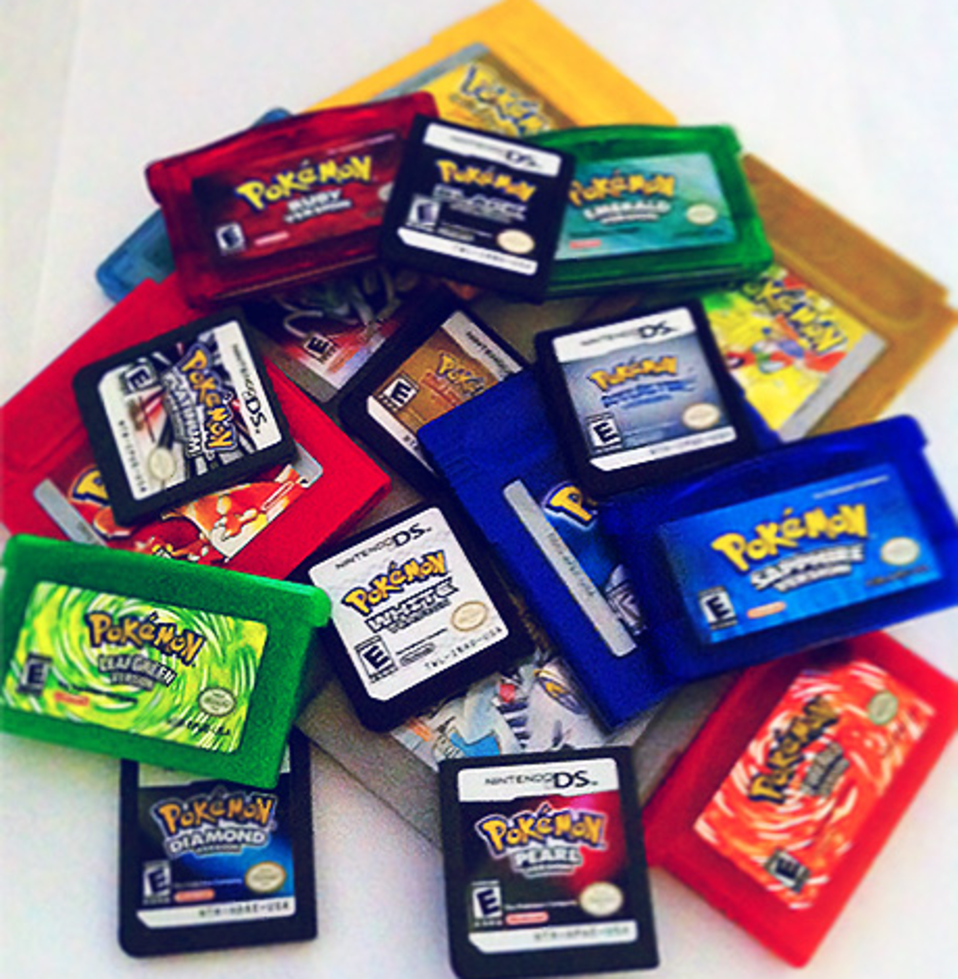
\includegraphics[width=\textwidth]{imgs/pokemon_cart.pdf}
  \end{column}
\end{columns}

\end{frame}


\begin{frame}{Metodología}

\end{frame}

\begin{frame}[fragile]{Cifrado XOR en Pokémon Perla y Diamante}
\begin{columns}
\begin{column}{0.75\textwidth}
    Textos: codificados y cifrados
    \begin{uncoverenv}<2->\begin{lstlisting}
ushort clave = 0x91BD3 * (num + 1);
for (int i=0; i<data.Length; i++){
  data[i] = data[i] ^ clave;
  clave = (ushort)(clave + 0x493D);
}
    \end{lstlisting}\end{uncoverenv}
\note<1>[item]{En la memoria se comenta un fallo de seguridad en el formato.}

    \uncover<3->{Imágenes: cifrado del bloque de datos}
    \begin{uncoverenv}<4->\begin{lstlisting}
uint clave = data[data.Length - 1];
for (int i=data.Length - 1; i>=0; i--){
  data[i] = data[i] ^ clave;
  clave = (uint)(clave * 0x41C64E6D + 0x6073);
}
    \end{lstlisting}\end{uncoverenv}
\end{column}

\begin{column}{0.25\textwidth}
    \visible<3->{
\includegraphics[width=\textwidth]{imgs/pearl_img_enc.png}}
    \vfill
    \visible<5->{
\includegraphics[width=\textwidth]{imgs/pearl_img_dec.png}}
\end{column}
\end{columns}
\end{frame}

\begin{frame}[fragile]{Archivos ofuscados en Pokémon Blanco y Negro}
\begin{columns}
\begin{column}{0.25\textwidth}
    \visible<2->{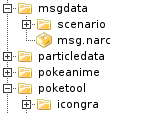
\includegraphics[width=\textwidth]{imgs/pearl_ofus_files.png}}
    \vfill
    \visible<3->{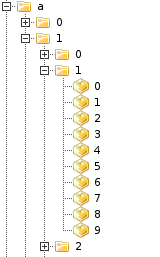
\includegraphics[width=\textwidth]{imgs/bw_ofus_files.png}}
\end{column}

\begin{column}{0.75\textwidth}
    \begin{itemize}
        \item<1-> Archivos ofuscados:
        \begin{itemize}
            \item<3-> Sin nombre ni clasificación.
        \end{itemize}

        \item<4-> Textos:
        \begin{itemize}
            \item<5-> Codificación \texttt{UTF-16}.
            \item<6-> Cifrado \texttt{XOR}, moviendo 3 bits de la clave.
        \end{itemize}

    \begin{uncoverenv}<6->\begin{lstlisting}
ushort clave = (num + 3) * 0x2983;
for (int i=0; i<data.Length; i++){
  data[i] = data[i] ^ clave;
  ushort temp = clave & 0x1FFF;
  clave = (temp<<3) | (clave>>13)
}
    \end{lstlisting}\end{uncoverenv}

        \item<7-> Imágenes:
            \begin{itemize}
                \item<8-> Cambio de formato.
            \end{itemize}
        \visible<8->{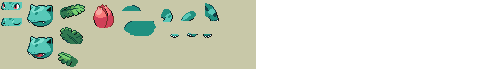
\includegraphics[width=\textwidth,height=0.8\textheight,keepaspectratio]{imgs/bw_image.png}}
    \end{itemize}
\end{column}
\end{columns}
\end{frame}

\subsection{}
\begin{frame}{Mecanismos en otros juegos}
Algoritmos de protección encontrados en otros juegos:

\begin{wideitemize}
    \item<+-> \textit{Pokémon HeartGold y SoulSilver}: Igual que \textit{Pokémon Perla y Diamante}.

    \item<+-> \textit{Pokémon Conquest}: Cifra y codifica textos. Imágenes con formatos no estándar.

    \item <+-> \textit{Ninokuni - El Mago de las Tinieblas}: Cifra estadísticas de personajes y monstruos. Añade algoritmos de integridad en el archivo de guardado.
\end{wideitemize}
\end{frame}
